\def\mytitle{OPTIMISATION}
\def\myauthor{Uday Kumar}
\def\contact{immadisettyudaykumar15@gmail.com}
\def\mymodule{Future Wireless Communication (FWC)}
\documentclass[10pt, a4paper]{article}
\usepackage[a4paper,outer=1.5cm,inner=1.5cm,top=1.75cm,bottom=1.5cm]{geometry}
\twocolumn
\usepackage{graphicx}
\graphicspath{{./images/}}
\usepackage[colorlinks,linkcolor={black},citecolor={blue!80!black},urlcolor={blue!80!black}]{hyperref}
\usepackage[parfill]{parskip}
\usepackage{lmodern}
\usepackage{tikz}
%\usepackage{physics}
%\documentclass[tikz, border=2mm]{standalone}
%\usepackage{karnaugh-map}
%\documentclass{article}
\usepackage{tabularx}
\usepackage{circuitikz}
\usetikzlibrary{calc}
\usepackage{amsmath}
\usepackage{amssymb}
\renewcommand*\familydefault{\sfdefault}
\usepackage{watermark}
\usepackage{lipsum}
\usepackage{xcolor}
\usepackage{listings}
\usepackage{float}
\usepackage{titlesec}
\newcommand{\myvec}[1]{\ensuremath{\begin{pmatrix}#1\end{pmatrix}}}
\newcommand{\mydet}[1]{\ensuremath{\begin{vmatrix}#1\end{vmatrix}}}
\providecommand{\brak}[1]{\ensuremath{\left(#1\right)}}
\providecommand{\lbrak}[1]{\ensuremath{\left(#1\right.}}
\providecommand{\rbrak}[1]{\ensuremath{\left.#1\right)}}
\providecommand{\sbrak}[1]{\ensuremath{{}\left[#1\right]}}
\providecommand{\mtx}[1]{\mathbf{#1}}
\titlespacing{\subsection}{1pt}{\parskip}{3pt}
\titlespacing{\subsubsection}{0pt}{\parskip}{-\parskip}
\titlespacing{\paragraph}{0pt}{\parskip}{\parskip}
\newcommand{\figuremacro}[5]{
    \begin{figure}[#1]
        \centering
   
        \includegraphics[width=#5\columnwidth]{#2}
        \caption[#3]{\textbf{#3}#4}
        \label{fig:#2}
    \end{figure}
}
\let\vec\mathbf
\lstset{
frame=single, 
breaklines=true,
columns=fullflexible
}

\title{\mytitle}
\author{\myauthor\hspace{1em}\\\contact\\FWC22086\hspace{6.5em}IITH\hspace{0.5em}\mymodule\hspace{6em}MATRICES}
\date{}
\begin{document}
\maketitle
\paragraph*{\large Problem statement}
\paragraph*{A wire of length 2 units is cut into two parts which are bent respectively to form a square of side 'a' units and a circle of radius ;r; units .If the sum of areas of the square and the circle so formed is minimum then :}
\textbf{To Find:} 
The relation between the radius of circle and side length 

\noindent \textbf{Given:} \\
Length of the wire is 2 units
\section{Construction}
   \begin{center}
  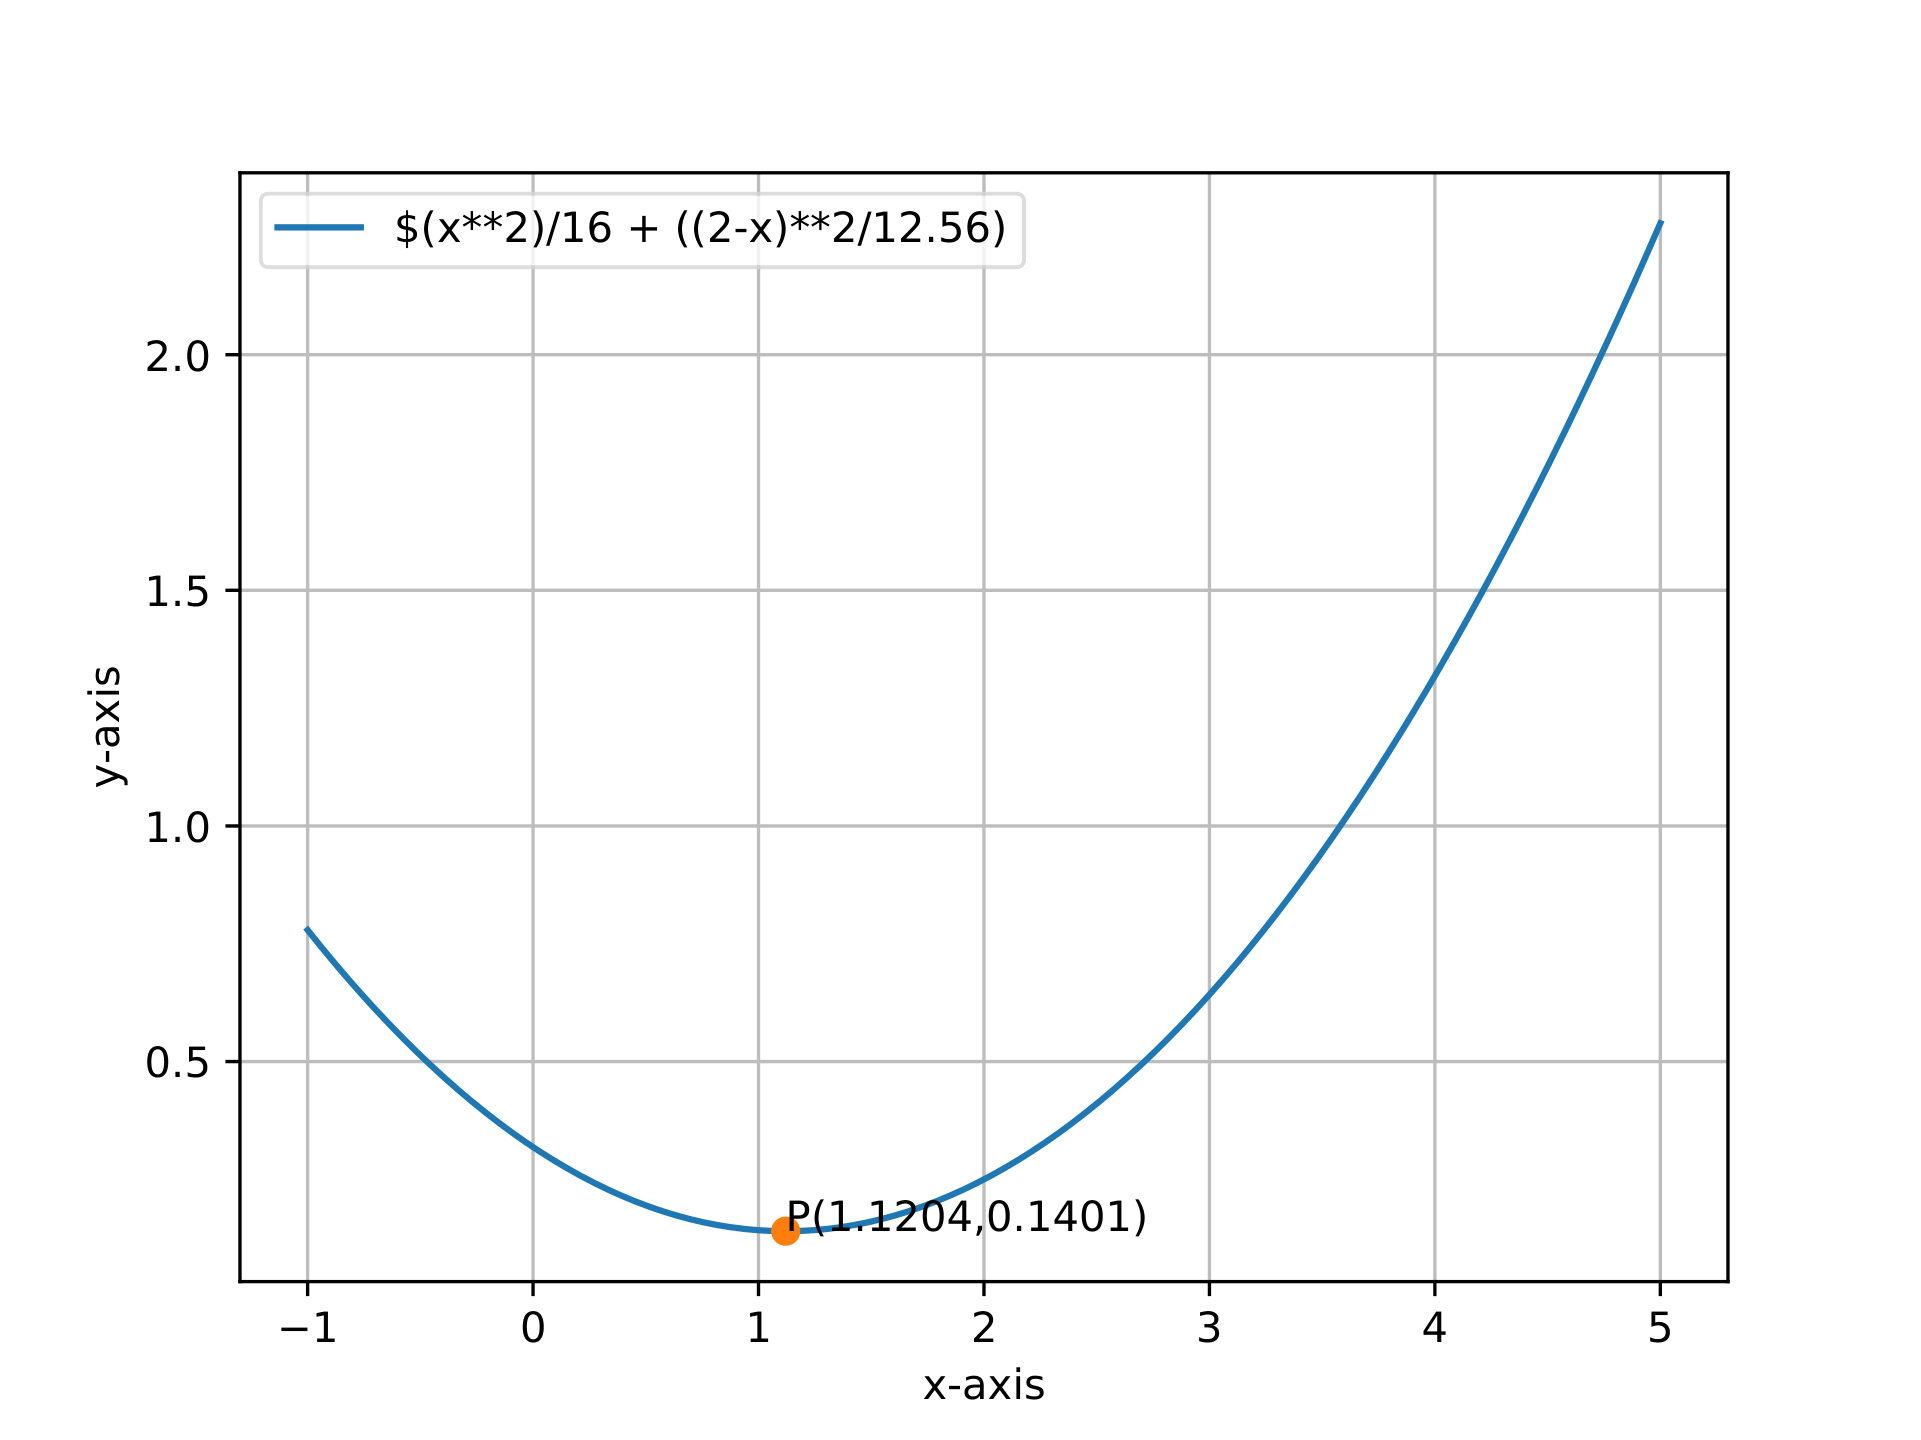
\includegraphics[scale=0.5]{optii.png}
    \end{center}
\section{solution}
\begin{equation}
\text{perimeter of the square is} \quad \vec{x} \quad \text{units} .
\end{equation} 
\begin{equation}
\text{circumfernce of circle is }\quad(2-x) \quad\text{units}.
\end{equation} 
\begin{equation}
\text{side length of square a = } x/4 \\
\label{eq-1}
\end{equation}

\begin{equation}
\text{radius  of the circle }
r=\frac{2-x}{2\pi}
\label{eq-2}
\end{equation}


So, the total length is 
\begin{equation}
4x + 2\pi r = 2
\end{equation} 

Now by using the formula for the area of the circle and square is:
\begin{equation}
\text{Area of square= }a^2
\end{equation}
\begin{equation}
\text{Area of the circle= }\pi r^2
\end{equation}
Now, the combined area(A) 
\begin{equation}
A=a^2+\pi r^2
\end{equation}
\begin{equation}
A = \frac{x^2}{16} + \frac{(2-x)^2}{4\pi}
\end{equation}
\textbf{Objective function:}
\begin{align}
A= \min_x\frac{x^2}{16} + \frac{(2-x)^2}{4\pi}\\
\end{align}
\textbf{constraints:}\\
\begin{center}
x$>$0\\
\end{center}



\section{Calculation of Minima using Gradient Descent algorithm}
\textbf{minima using  Gradient Descent  method}
The minimum value is caluculated by using gradient descent method.
\begin{align}
        x_{n+1} &= x_n - \alpha \nabla A(x_n) \\
        \implies x_{n+1} &= x_n - \alpha\brak{\frac{x}{8}-\frac{2-x}{6.28}}
\end{align}
where \\
\begin{enumerate}
\item $\alpha$ = 0.001
\item $x_{n+1}$ is current value
\item $x_{n}$ is previous value
\item precession = 0.00000001
\item maximum iterations = 100000000
\end{enumerate}
The combined area has minimum value at 1.1204 i.e
\begin{equation}
\frac{8}{4+\pi}
\end{equation}

The  combined area is minimum with side length a is 
\begin{equation}
a =\frac{2}{4+\pi}
\end{equation}
The area of the circle is minimum with radius 
\begin{equation}
r =\frac{1}{4+\pi}
\end{equation}
Hence, the 
\begin{equation}
\boxed{$a = 2r$}
\end{equation}
\end{document}
